\chapter{Podstawy teoretyczne} \label{chap:teoria}
W tym rozdziale zostaną omówione podstawowe pojęcia związane z tematem pracy. Pierwsze dwa podrozdziały skupiają się na opisie czym w ogóle jest aplikacja internetowa, oraz opisują jedno z najpopularniejszych podejść do budowania aplikacji internetowej, SPA. W kolejnych podrozdziałach zostały opisane technologie, które są porównywane w dalszej części pracy.
\section{Aplikacja internetowa}
Aplikacja internetowa jest czymś więcej niż zwykłą stroną internetową. Z definicji jest to aplikacja typu klient-serwer, w której klient jest uruchamiany przy pomocy przeglądarki internetowej. Oprogramowanie klienta jest pobierane na komputer klienta podczas wizyty na odpowiedniej stronie internetowej, przy użyciu standardowych procedur, takich jak HTTP. Aktualizacje oprogramowania klienta mogą odbywać się za każdym razem, gdy odwiedzana jest strona internetowa. W czasie trwania sesji przeglądarka internetowa interpretuje i wyświetla strony, oraz działa jako uniwersalny klient dla dowolnej aplikacji internetowej.
\begin{figure}[h]
	\centering
	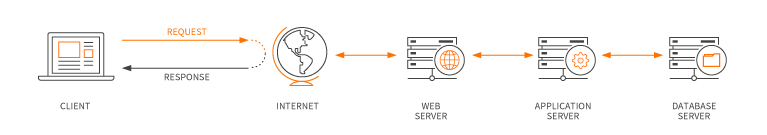
\includegraphics[width=\textwidth]{images/how_web_application_works}
	\caption{Podstawowy schemat działania aplikacji internetowej \cite{MaxCdnWebApp}}
\end{figure}
%\subsection{Krótki rys historyczny}
\section{SPA}
Skrót SPA pochodzi od \textit{Single-page Application}. Jest to aplikacja internetowa działająca wewnątrz przeglądarki, która podczas użytkowania strony nie wymaga odświeżania strony. W tym podejściu, cały niezbędny kod źródłowy -- HTML, JavaScript i CSS -- jest pobierany przy pojedyńczym załadowaniu strony, lub odpowiednie zasoby są ładowane dynamicznie i dodawane do strony jedynie wtedy, kiedy jest to potrzebne. Idea jaka stoi za takim rozwiązaniem, to przede wszystkim lepszy, bardziej naturalny user expierience. Użytkownik po wejściu na stronę, nie musi przy każdej interakcji oczekiwać na ponowne załadowanie się strony, czy też jej odświeżanie.

\begin{figure}[h]
	\centering
	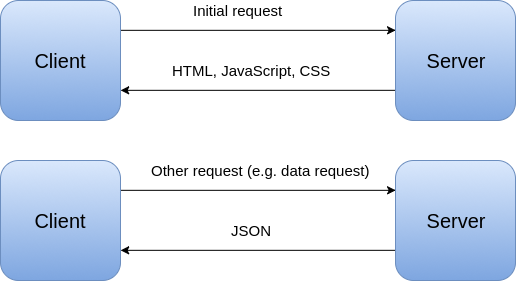
\includegraphics[width=0.6\textwidth]{images/spa}
	\caption{Podstawowy schemat działania aplikacji internetowej \cite{MaxCdnWebApp}}
\end{figure}

Choć koncept SPA zaczął być częściej używany po spopularyzowaniu AJAX'a\footcite{Asynchronous JavaScript And XML}, to tak naprawdę dopiero od kilku lat jest on powszechnie wykorzystywany podczas budowania aplikacji internetowych. Serwisy takie jak Gmail, Google Maps, Facebook czy GitHub są właśnie aplikacjami typu single-page application. Także większość najpopularniejszych bibliotek JavaScript'owych umożliwiają implementację aplikacji internetowej zgodnie z zasadami SPA.
\subsection{Zalety}
\begin{itemize}
	\item Szybkość działania - większość zasobów jest ładowana tylko raz podczas cyklu życia aplikacji, jedynymi informacjami, które są wymieniane z serwerem cały czas, są dane
	\item Brak ciągłego przeładowywania strony
	\item Znacznie prostszy proces wdrożenia aplikacji - jedyne co jest potrzebne to statyczny serwer serwujący minimalnie 3 pliki - pojedynczą stronę HTML, oraz 2 pakiety: jeden zawierający wszystkie style, drugi skupiający w sobie cały kod JavaScriptow'y
	\item Odciążenie strony serwerowej - serwer zamiast generować za każdym razem pełny kod strony, transmituje jedynie potrzebne w danej chwili dane.
\end{itemize}
\subsection{Wady}
\begin{itemize}
	\item Powolne początkowe uruchomienie strony - wymaga ono załadowania framework'u, oraz przynajmniej części aplikacji, która później już nie jest ponownie ściągana.
	\item Ze względu na zależność SPA od JavaScript'a, bardzo łatwo o pojawienie się wycieków pamięci pomiędzy długimi okresami czasu między przeładowaniami strony
	\item
\end{itemize}

\section{JavaScript}

\section{React.js}

\section{Redux}

\section{Elm}